\documentclass[aspectratio=169,10pt]{beamer}

\usetheme{Madrid}
\usecolortheme{seahorse}
\usepackage{booktabs}
\usepackage{colortbl}
\usepackage{amsmath}
\usepackage{amssymb}
\usepackage{xcolor}
\usepackage{tikz}
\usepackage{microtype}

\definecolor{mynavy}{HTML}{1B2A4A}
\definecolor{myteal}{HTML}{009B77}
\definecolor{mylgray}{HTML}{F0F2F5}
\definecolor{mydgray}{HTML}{444455}
\definecolor{mydgreen}{HTML}{007A5E}
\definecolor{myhighlight}{HTML}{D4EDDA}

\setbeamercolor{palette primary}{bg=mynavy,fg=white}
\setbeamercolor{palette secondary}{bg=mynavy!80,fg=white}
\setbeamercolor{palette tertiary}{bg=mynavy!60,fg=white}
\setbeamercolor{palette quaternary}{bg=mynavy,fg=white}
\setbeamercolor{structure}{fg=mynavy}
\setbeamercolor{alerted text}{fg=myteal}
\setbeamercolor{block title}{bg=mynavy,fg=white}
\setbeamercolor{block body}{bg=mylgray,fg=mydgray}
\setbeamercolor{block title alerted}{bg=myteal,fg=white}
\setbeamercolor{block body alerted}{bg=myteal!10,fg=mydgray}
\setbeamerfont{frametitle}{series=\bfseries,size=\large}
\setbeamerfont{block title}{series=\bfseries}
\setbeamertemplate{navigation symbols}{}
\setbeamertemplate{itemize items}[circle]

\newcommand{\hl}[1]{\textcolor{myteal}{\textbf{#1}}}

\title[Pedagogical Friction Detector]{Multimodal Pedagogical Friction Detector}
\subtitle{Fusing Facial Affect $\cdot$ Talk Moves $\cdot$ LLM Reasoning\\
          to Surface Teachable Moments at Scale}
\author{Jingrui Wu}
\institute{Rice University $\cdot$ COMP 646}
\date{2026}

\begin{document}

\begin{frame}[plain]
  \titlepage
\end{frame}

%------------------------------------------------------------
\begin{frame}{Slide 1 / 5 \quad Motivation}
\begin{alertblock}{Why this problem?}
Manual classroom coding takes years of expert effort and cannot scale to
real-time teacher feedback~\cite{timss1999video}.
\end{alertblock}
\medskip
\begin{columns}[T]
\column{0.49\textwidth}
\textbf{\textcolor{myteal}{The challenge}}
\begin{itemize}
  \item When students are confused, the teacher's \textbf{next move} is
        critical for deep learning \cite{dmello2012}
  \item Existing tools are \textbf{single-modal}: transcript \emph{or}
        affect --- never fused with semantic reasoning
  \item Edu-ConvoKit \& TutorCoPilot ignore student affect;
        affect systems ignore teacher response quality
\end{itemize}
\column{0.49\textwidth}
\textbf{\textcolor{myteal}{Our goal}}
\begin{itemize}
  \item Define \hl{Pedagogical Friction}: elevated student confusion
        \textbf{and} a low-quality teacher move in the same 30-second window
  \item Fuse \textbf{vision} (DeepFace) $+$ \textbf{language}
        (ELECTRA $+$ \texttt{claude-sonnet-4-6})
  \item Scale to \hl{53 TIMSS lessons, 7 countries} without human labelling
\end{itemize}
\end{columns}
\end{frame}

%------------------------------------------------------------
\begin{frame}{Slide 2 / 5 \quad Problem Setup}
\begin{block}{Definition of Pedagogical Friction}
A 30-second window where student confusion is \emph{elevated} \textbf{AND}
the teacher's talk move is \emph{low-quality} (answer-giving, closed loops,
transmission-only instruction).
\end{block}
\bigskip
\begin{columns}[T]
\column{0.31\textwidth}
\textbf{\textcolor{myteal}{Video data}}
\begin{itemize}
  \item TIMSS AU1 lesson (10 min)
  \item 1\,200 frames $\to$ DeepFace @ 2\,Hz
  \item 87 bins $|$ 1 human positive
\end{itemize}
\column{0.33\textwidth}
\textbf{\textcolor{myteal}{Transcript corpus}}
\begin{itemize}
  \item 53 TIMSS lessons
  \item 28 math + 25 science
  \item 7 countries $|$ 5\,113 bins
\end{itemize}
\column{0.33\textwidth}
\textbf{\textcolor{myteal}{Annotation}}
\begin{itemize}
  \item Human: 1 positive (bin\,11)
  \item Heuristic: 31.5\% flagged
  \item ELECTRA: 19.3\% flagged
\end{itemize}
\end{columns}
\bigskip
\begin{alertblock}{}
\centering\textbf{Shared 30-second temporal grid} aligns vision \&
language streams for every lesson.
\end{alertblock}
\end{frame}

%------------------------------------------------------------
\begin{frame}{Slide 3 / 5 \quad Pipeline Architecture}
\begin{center}
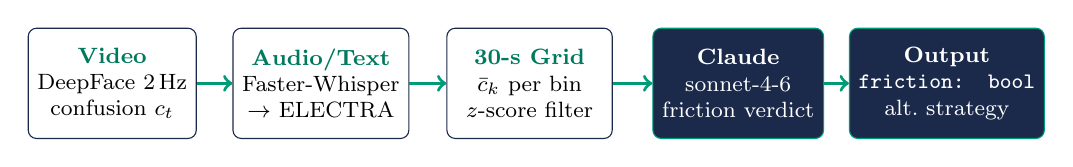
\begin{tikzpicture}[
  box/.style={draw=mynavy,fill=white,rounded corners=3pt,
              minimum width=2.1cm,minimum height=1.4cm,
              align=center,font=\footnotesize},
  darkbox/.style={draw=myteal,fill=mynavy,rounded corners=3pt,
                  minimum width=2.1cm,minimum height=1.4cm,
                  align=center,font=\footnotesize,text=white},
  arr/.style={->,very thick,color=myteal}]
\node[box]     (V) at (0,0)     {\textcolor{mydgreen}{\textbf{Video}}\\\footnotesize DeepFace 2\,Hz\\confusion $c_t$};
\node[box]     (L) at (2.65,0)  {\textcolor{mydgreen}{\textbf{Audio/Text}}\\\footnotesize Faster-Whisper\\\footnotesize$\to$ ELECTRA};
\node[box]     (G) at (5.3,0)   {\textcolor{mydgreen}{\textbf{30-s Grid}}\\\footnotesize$\bar{c}_k$ per bin\\$z$-score filter};
\node[darkbox] (C) at (7.95,0)  {\textbf{Claude}\\\footnotesize sonnet-4-6\\friction verdict};
\node[darkbox] (O) at (10.6,0)  {\textbf{Output}\\\footnotesize\texttt{friction: bool}\\alt.\ strategy};
\draw[arr] (V)--(L); \draw[arr] (L)--(G);
\draw[arr] (G)--(C); \draw[arr] (C)--(O);
\end{tikzpicture}
\end{center}
\vspace{-0.5em}
\begin{columns}[T]
\column{0.48\textwidth}
\textbf{\textcolor{myteal}{Confusion proxy (Eq.\,1)}}
\[c_t=\textstyle\sum_{e\in\mathcal{E}}w_e\cdot p_t(e)\]
{\footnotesize$w_{\text{fear}}{=}0.90,\;w_{\text{sad}}{=}0.85,\;w_{\text{disgust}}{=}0.50$\ldots}
\column{0.48\textwidth}
\textbf{\textcolor{myteal}{Candidate filter (Eq.\,2)}}
\[\bar{c}_k>\mu_C+z\,\sigma_C\;\wedge\;q_k\neq\textit{high}\]
{\footnotesize$z{=}1.0$ flags the top $\sim$16\% of bins.}
\end{columns}
\smallskip
\begin{alertblock}{}
\small Talk Move fallback:\quad
\textbf{(1)}~ELECTRA $\to$ \textbf{(2)}~Edu-ConvoKit $\to$ \textbf{(3)}~Keyword heuristic
\end{alertblock}
\end{frame}

%------------------------------------------------------------
\begin{frame}{Slide 4 / 5 \quad Experiments}
\begin{columns}[T]
\column{0.32\textwidth}
\begin{block}{\small Track 1: AU1 Full Video}
\begin{itemize}\footnotesize
  \item 1\,200 frames $\to$ DeepFace + Whisper + Claude
  \item 7 candidates $\to$ Claude rejects \textbf{all} (social disruption)
  \item Wide-angle: $\bar{c}_k{=}0$ every bin --- \textbf{vision fails}
\end{itemize}
\end{block}
\column{0.32\textwidth}
\begin{block}{\small Track 2: 54-Lesson Scale-Up}
\begin{itemize}\footnotesize
  \item SLURM GPU array (NVIDIA A40)
  \item 5\,318 bins $|$ 1\,797 flagged
  \item Claude confirms \textbf{21} moments (0.4\%)
  \item Wide-angle failure confirmed
\end{itemize}
\end{block}
\column{0.33\textwidth}
\begin{block}{\small Track 3: Human Eval (87 bins)}
\begin{itemize}\footnotesize
  \item 1 annotator $\to$ \textbf{1 positive} (bin\,11)
  \item Heuristic: F1\,=\,0.10
  \item ELECTRA: F1\,=\,0.00
  \item Heuristic + Claude: \hl{F1\,=\,1.00}
\end{itemize}
\end{block}
\end{columns}
\bigskip
\begin{alertblock}{Key finding}
$r{=}{-}0.35$ correlation between heuristic \& ELECTRA rates across
53 lessons $\Rightarrow$ \textbf{annotation methodology is a first-class design variable}.
\end{alertblock}
\end{frame}

%------------------------------------------------------------
\begin{frame}{Slide 5 / 5 \quad Results \& Takeaways}
\begin{columns}[T]
\column{0.54\textwidth}
{\small
\begin{tabular}{lrrrr}
\toprule
\textbf{Condition} & \textbf{Bins} & \textbf{Flag} & \textbf{\%} & \textbf{F1}\\
\midrule
\multicolumn{5}{l}{\textit{Human evaluation (AU1, 87 bins)}}\\
\quad Heuristic           &  87 &  20 & 23\% & 0.10 \\
\quad ELECTRA             &  87 &  33 & 38\% & 0.00 \\
\rowcolor{myhighlight}
\quad + Claude            &  87 &   1 &  1\% & \textbf{1.00} \\
\midrule
\multicolumn{5}{l}{\textit{Transcript-only (53 lessons)}}\\
\quad Heuristic           & 5113 & 1611 & 31.5\% & --- \\
\quad ELECTRA             & 5113 &  988 & 19.3\% & --- \\
\rowcolor{myhighlight}
\quad + Claude            & 5113 &  211 &  4.1\% & --- \\
\bottomrule
\end{tabular}
}
\column{0.44\textwidth}
\begin{itemize}\setlength\itemsep{0.5em}
  \item[\hl{$\star$}] \textbf{F1\,=\,1.00}\\
        Claude cuts false positives $20\times$; zero missed detections
  \item[\hl{$\star$}] \textbf{7.6$\times$ reduction}\\
        1\,611 flags $\to$ 211 confirmed friction moments
  \item[\hl{$\star$}] \textbf{$r{=}{-}0.35$}\\
        Heuristic vs ELECTRA anti-correlated across 7 countries
  \item[\hl{$\star$}] \textbf{Vision limit}\\
        Wide-angle $\Rightarrow$ DeepFace unusable;
        language is the primary signal
\end{itemize}
\end{columns}
\end{frame}

%------------------------------------------------------------
\begin{frame}[allowframebreaks]{References}
{\footnotesize
\bibliographystyle{ieeetr}
\bibliography{egbib}
}
\end{frame}

\end{document}
